%%%%%%%%%%%%%%%%%%%%%%%%%%%%%%%%%%%%%%%%%%%%%%%%%%%%%%%%%%%%
%%% ELIFE ARTICLE TEMPLATE
%%%%%%%%%%%%%%%%%%%%%%%%%%%%%%%%%%%%%%%%%%%%%%%%%%%%%%%%%%%%
%%% PREAMBLE 
\PassOptionsToPackage{table}{xcolor}
%\documentclass[9pt,lineno]{elife}
\documentclass[9pt,lineno]{elife-modified} % use modified template
% Use the onehalfspacing option for 1.5 line spacing
% Use the doublespacing option for 2.0 line spacing
% Please note that these options may affect formatting.

\usepackage{lipsum} % Required to insert dummy text
\usepackage[version=4]{mhchem}
\usepackage{siunitx}
\DeclareSIUnit\Molar{M}
\usepackage{tabularx}
\usepackage[numbers,sort&compress,square]{natbib}

% Use sans serif for math throughout
%\usepackage{sansmathfonts} % There seems to be something wrong with incorrect symbols showing up 

\usepackage[colorinlistoftodos,prependcaption,textsize=tiny]{todonotes}
\definecolor{forestgreen}{RGB}{10, 67, 28}
\usepackage{soul}

\usepackage{rotating} %rotate wide tables sideways :: sidewaystable --> \begin{sidewaystable}... == \begin{table}...

%%%%%%%%%%%%%%%%%%%%%%%%%%%%%%%%%%%%%%%%%%%%%%%%%%%%%%%%%%%%
%%% ARTICLE SETUP
%%%%%%%%%%%%%%%%%%%%%%%%%%%%%%%%%%%%%%%%%%%%%%%%%%%%%%%%%%%%

\title{Is structure based drug design ready for selectivity optimization?}  %%% 9/15 words


\author[1,2]{Steven K. Albanese}
\author[2]{John D. Chodera}
\author[3]{Simon Peng}
\author[3]{Robert Abel}

\author[3*]{Lingle Wang}


\affil[1]{Louis V. Gerstner, Jr. Graduate School of Biomedical Sciences, Memorial Sloan Kettering Cancer Center, New York, NY 10065}
\affil[2]{Computational and Systems Biology Program, Sloan Kettering Institute, Memorial Sloan Kettering Cancer Center, New York, NY 10065}
\affil[3]{Schr\"{o}dinger, New York, NY 10036}


\corr{lingle.wang@schrodinger.com}{LW}

%%%%%%%%%%%%%%%%%%%%%%%%%%%%%%%%%%%%%%%%%%%%%%%%%%%%%%%%%%%%
%%% ARTICLE START
%%%%%%%%%%%%%%%%%%%%%%%%%%%%%%%%%%%%%%%%%%%%%%%%%%%%%%%%%%%%

\begin{document}

\maketitle

%
%
%  ABSTRACT
%
%
\begin{abstract}
%%% /150 words

Alchemical free energy calculations are now widely used to drive or maintain potency in small molecule lead optimization, where the binding affinity to a protein target can be computed---in well-behaved cases---to roughly 1 kcal/mol inaccuracy, which is believed to primarily stem from force field errors.
Despite this, the potential to use free energy calculations to drive optimization of compound \emph{selectivity} among two similar targets has been relatively unexplored.
In the most optimistic scenario, the similarity of binding sites might lead to a fortuitous cancellation of force field errors and allow selectivity to be predicted more accurately than affinity.
Here, we assess the accuracy with which selectivity can be predicted in the context of small molecule kinase inhibitors, considering the very similar binding sites of human kinases CDK2 and CDK9, as well as another series of ligands attempting to achieve selectivity between the more distantly related kinases CDK2 and ERK2.
Using a novel Bayesian analysis approach, we separate force field error from statistical error and quantify the correlation in force field errors between selectivity targets.
We find that, in the closely related CDK2/CDK9 case, a high correlation in force field errors suggests free energy calculations can have significant impact in aiding chemists in achieving selectivity, while in more distantly related kinases (CDK2/ERK2), limited correlation in force field errors reduces the ability for free energy calculations to aid selectivity optimization.
In both cases, the correlation in force field error suggests that longer simulations are beneficial to properly balance statistical error with systematic error to take full advantage of the increase in accuracy in selectivity prediction possible due to fortuitous cancellation of error.

\end{abstract}


%
%
%  INTRODUCITON (want to see if this works) 
%
%
Free energy methods have proven useful in aiding structure-based drug design by driving the optimization or maintenance of potency in lead optimization. Alchemical free energy calculations allow for prediction of ligand binding free energies, including all enthalpic and entropic contributions~\citep{Chodera2011-jn}. Advances in atomistic molecular mechanics forcefields and free energy methodologies~\citep{Huang:J.Comput.Chem.:2013,Maier:J.Chem.TheoryComput.:2015,Harder:J.Chem.TheoryComput.:2016,Cournia:2017ip} have allowed free energy methods to reach a level of accuracy  sufficient for predicting ligand potencies~\citep{BROWN2009420}. Free energy methods have been applied prospectively to develop inhibitors for Tyk2~\citep{Abel2017-gw}, Syk~\citep{Lovering:2016fg}, BACE1~\citep{Ciordia:2016dn}, GPCRs~\citep{Lenselink:2016ip}, and HIV protease~\citep{Jorgensen:2016dv}. A recent large-scale review found that the use of FEP+~\citep{Wang:J.Am.Chem.Soc.:2015} to predicting potency for 92 different projects and 3021 compounds found a median RMSE of 1 kcal/mol~\citep{Abel:2017jt}. 

\paragraph{Selectivity is an important consideration in drug design}
In addition to maintaining or optimizing potency, free energy methods can be applied to predicting the selectivity of a ligand between two or more targets. Selectivity is an important property to consider in drug development, either in the pursuit of a maximally selective inhibitor~\citep{Zhang2009-il,Huggins2012-hr} or in pursuit a polypharmacological agent~\citep{Fan2007-hm,Apsel2008-it,Knight:Nat.Rev.Cancer:2010,Hopkins2006-qu,Hopkins2008-ij}, to avoid on-target toxicity (arising from inhibition of the intended target)~\citep{Rudmann2013-hi}  and off-target toxicity (arising from inhibition of unintended targets)~\citep{Kijima2011-xs,Liu2014-yi}. In either paradigm, considering the selectivity of a compound is complicated by the biology of the target. For example, kinases exist as nodes in complex signaling networks~\citep{Mendoza2011-bj,Tricker2015-xx} with feedback inhibition and cross-talk between pathways. Careful consideration of which off-targets are being inhibited can avoid off-target toxicity due to alleviating feedback inhibition and inadvertently reactivating the targeted pathway~\citep{Mendoza2011-bj,Tricker2015-xx}, or the upregulation of a secondary pathway by alleviation of cross-talk inhibition~\citep{Bailey2014-pd,Chandarlapaty:CancerCell:2011}. Off-target toxicity can also be caused by inhibiting unrelated targets, such as gefitinib, an EGFR inhibitor, inhibiting CYP2D6~\citep{Kijima2011-xs} and causing hepatotoxicity in lung cancer patients. In a cancer setting, on-target toxicity can be avoided by considering the selectivity for the oncogenic mutant form of the kinase over the wild type form of the kinase~\citep{Pao2004-kx,Kim2012-mo,Juchum:DrugResist.Updat.:2015}, demonstrated by number of first generation EGFR inhibitors. Selectivity considerations can also lead to beneficial effects: Imatinib, intially developed to target BCR-Abl fusion proteins, is also approved for treating gastrointestinal stromal tumors (GIST)~\citep{Din2008-ag} due to its activity against receptor tyrosine kinase KIT. 

\paragraph{Use of physical modeling to predict selectivity is relatively unexplored}
While predicting selectivity is important for drug discovery, but the utility of free energy methods for predicting this property is relatively unexplored. If there is fortuitous cancellation of errors for closely related systems, free energy methods may be much more accurate than expected given the errors made in predicting the potency for each individual target. The selectivity of Imatinib for Abl kinase over Src~\citep{Lin2013-ft,Lin2014-iv} and within a family of non-receptor tyrosine kinases~\citep{Lin2013-mu} has been studied extensively using molecular dynamics and free energy calculations. This work focuses on understanding the role reorganization energy plays in the exquisite selectivity of imatinib for Abl over Src despite high similarity between cocrystallized binding mode and kinase conformations, and does not touch on the evaluation of the accuracy of these methods, or their application to drug discovery on congeneric series of ligands. Previous work predicting the selectivity of three bromodomain inhibitors accross the bromodomain family achieved promising accuracy for single target potencies of roughly 1 kcal/mol, but does not explicitly evaluate any selectivity metrics~\citep{Aldeghi2017-ox} or look at correlation in the errors made for each bromodomain. 


\paragraph{Kinases are an interesting and particularly challenging model system for selectivity predictions}
Kinases are a useful model system to work with for assesing the utility of free energy calculations to predict selectivity. With the approval of imatinib for the treatment of chronic myelogenous leukemia in 2001, targeted small molecule kinase inhibitors (SMKIs) have become a major class of therapeutics in treating cancer and other diseases. 
Currently, there are 43 FDA-approved SMKIs~\citep{fda-approved-kinase-inhibitors}, and it is estimated that kinase targeted therapies account for as much as 50\% of current drug development~\citep{Santos:Nat.Rev.DrugDiscov.:2016}, with many more compounds currently in clinical trials. 
While there have been a number of successes, the current stable of FDA-approved kinase inhibitors targets only a small number of kinases implicated in disease, and the design of new selective kinase inhibitors remains a significant challenge.
Achieving desired selectivity profiles is particularly difficult for kinase targets, making them a system where physical modelling has the potential for a large impact. Achieving selective inhibition of kinases is challenging as there are more than 518 protein kinases~\citep{Volkamer2015-jx,Manning2002-cw} with a highly conserved ATP binding site that is targeted by the majority of SMKIs~\citep{Wu2015-oq}.
While kinase inhibitors have been designed to target kinase-specific subpockets and binding modes to achieve selectivity~\citep{Cowan-Jacob2007-rn,Seeliger2007-jn,Huse2002-ml,Harrison2003-ct,Volkamer2016-sj,ChristmannFranck:2016gka}, previous work has shown that both Type I (binding to the active, DFG-in conformation) and Type II (binding to the inactive, DFG-out conformation) inhibitors display a wide variety of selectivities~\citep{Anastassiadis2011-sm,Davis:Nat.Biotechnol.:2011}, often exhibiting significant binding a number of other targets in addition to their primary target. 
Even FDA-approved inhibitors---often the result of extensive drug development programs---bind to a large number of off-target kinases~\citep{Klaeger2017-jr}. Kinases are also targets of interest for developing polypharmacological compounds, or inhibitors that are specifically designed to inhibit multiple kinase targets. Resistance to MEK inhibitors in KRAS-mutant lung and colon cancer has been shown to be driven by HER3 upregulation~\citep{Sun:2014kt}, providing rational for dual MEK/ERBB family inhibitors. Similarly, combined MEK and VEGFR1 inhibition has been proposed as a combinatorial approach to treat KRAS-mutant lung cancer~\citep{Manchado:2016fb}. Developing inhibitors with the desired polypharmacology means navigating more complex selectivity profiles. In well-behaved kinase systems, free energy calculations potency predictions have achieved mean unsigned errors of less than 1.0 kcal/mol~\citep{Wang:J.Am.Chem.Soc.:2015,Abel2017-gw}, suggesting that kinases can be computationally tractable as well as clinically interesting. 

\paragraph{Assessing the ability of alchemical free energy methods to predict selectivity}
We anticipate difficulty in predicting selectivity if the errors in the alchemical free energy calculations for two targets are largely uncorrelated, or even anticorrelated. However, correlation in the forcefield errors of the free energies for the two targets could lead to a fortuitous cancellation of errors in predicting the selectivity between targets, making selectivity predictions \emph{more} accurate than potency predictions. Such correlation could occur because the same chemical elements appear in the ligand and in highly related binding sites. 
Here, we investigate the magnitude of this correlation ($\rho$) and the utility of alchemical free energy calculations for the prediction of selectivity, hereafter taken to mean the $\Delta \Delta$G in binding free energies of the same compound for two targets. We employed state of the art relative free energy calculations~\citep{Wang:J.Am.Chem.Soc.:2015,Abel:2017jt} to predict the selectivities of two different congeneric ligand series~\citep{Shao2013-oe, Blake2016-su}, as well as present a simple numerical model to quantify the potential speed up in selectivity optimization expected for different combinations of per target errors and correlation coefficient values. To tease out the effects of a limited number of experimental measurements, we develop a new Bayesian approach to quantify the uncertainty in the correlation coefficient in the predicted change in selectivity on ligand modification, incorporating all sources of uncertainty and correlation in the computation to separate statistical from force field error. We find that in the closely related systems of CDK2 and CDK9, a high correlation of force field errors suggests that free energy methods can have a significant impact on speeding up selectivity optimization. In the more distantly related case (CDK2/ERK2), limited correlation hampers the ability for free energy methods to speed up selectivity optimization. 

   
%
%
%  RESULTS
%
%
\section{Methods}

\paragraph{Numerical model of selectivity}
To model the impact correlation would have on the expected uncertainty for selectivity predictions, $\sigma_{selectivity}$ was calculated using Equation~\ref{eq11} for 1000 evenly spaced values of the correlation coefficient ($\rho$) from 0 to 1, for a number of combinations of per target errors ($\sigma_{target1}$ and $\sigma_{target2}$) 

\begin{equation}\label{eq11}
\sigma_{selectivity} = \sqrt{\sigma_{target1}^2 + \sigma_{target2}^2 - 2\rho\sigma_{target1}\sigma_{target2}}
\end{equation}

The speed up in selectivity optimization that could be expected from using free energy calculations of a particular per target error ($\sigma_{selectivity}$) was quantify as follows using NumPy (v 1.14.2). An original, true distribution for the changed in selectivity of 200000000 new compounds proposed with respected to a reference compound was modeled as a normal distribution centered around 0 with a standard deviation of 1 kcal/mol. This assumption was made on the basis that the majority of selectivity is driven by the scaffold, and R group modifications will do little to drive changes in selectivity. The 1 kcal/mol distribution is supported by the standard deviations of the selectivity in the experimental datasets referenced in this work, which are all less than, but close, to 1 kcal/mol. 

Each of these proposed compounds were "screened" by a free energy calculation technique with a per target error ($\sigma_{target}$) of 1 kcal/mol~\citep{Wang:J.Am.Chem.Soc.:2015} and a specified correlation coefficient $\rho$. A $\sigma_{selectivity}$ was calculated according to Equation~\ref{eq11}. The noise of the computational method was modeled as a normal distribution centered around 0 with a standard deviation of $\sigma_{selectivity}$ and added to the "true" change in selectivity. Any compound predicted to have an improvement in selectivity of 1.4 kcal/mol (1 log unit) would then be made and have its selectivity experimental measured. The speedup value for each value of $\rho$ is calculated as the proportion of compounds made with a true selectivity gain of 1.4 kcal/mol divided by the proportion of compounds with a 1.4 kcal/mol improvement in the original distribution, where all of the compounds were made. 

Finally, this process was repeated for a 100x (2.8 kcal/mol, 2 log unit) selectivity optimization and 50 linearly spaced values of the correlation coefficient ($\rho$) between 0 and 1, for four values of $\sigma_{selectivity}$ and 40000000 compounds in the original distribution. 

\paragraph{Structure Preparation}
Structures from the Shao~\citep{Shao2013-oe} and Hole~\citep{Hole2013-sr}, and Blake~\citep{Blake2016-su} papers were downloaded from the PDB~\citep{Berman2002-hg},selecting structures with the same co-ligand crystallized. For the Shao dataset, 4BCK (CDK2) and 4BCI (CDK9) were selected, which have ligand 12c cocrystallized. For the Blake dataset, 5K4J (CDK2) and 5K4I (ERK2) were selected, cocrystallized with ligand 21. The structures were prepared using Schrodinger’s Protein Preparation Wizard~\citep{Sastry2013-ax} (release 2017-3). This pipeline modeled in internal loops and missing atoms, added hydrogens at the reported experimental pH (7.0 for the Shao dataset, 7.3 for the Blake dataset) for both the protein and the ligand. All crystal waters were retained. The ligand was assigned protonation and tautomer states using Epik at the experimental pH$\pm2$, and hydrogen bonding was optimized using PROPKA at the experimental pH$\pm2$. Finally, the entire structure was minimized using OPLS3 with an RMSD cutoff of 0.3\AA.

\paragraph{Ligand Pose Generation}
Ligands were extracted from the publication entries in the BindingDB as  2D SMILES strings. 3D conformations were generated using LigPrep with OPLS3~\citep{Harder2016-zn}. Ionization state was assigned using Epik at experimental pH$\pm2$. Stereoisomers were computed by retaining any specified chiralities and varying the rest. The tautomer and ionization state with the lowest epik state penalty was selected for use in the calculation. Ligand poses were generated by first aligning to the co-crystal ligand using the Largest Common Bemis-Murcko scaffold with fuzzy matching (Schrodinger 2017-4). Ligands that were poorly aligned or failed to align were then aligned using Maximum Common Substructure (MCSS). Finally, large R-groups were allowed to sample different conformations using MM-GBSA with a common core restrained. VSGB solvation model was used with the OPLS3 forcefield. No flexible residues were defined for the ligand. 

\paragraph{Free Energy Calculations}
The FEP+ panel (Maestro release 2017-4) was used to generate perturbation maps. Neutral perturbations were run for 15ns per replica, using an NPT ensemble and water buffer size of 5\AA. A GCMC solvation protocol was used to sample buried water molecules in the binding pocket prior to the calculation, which discards any retained crystal waters. 

\paragraph{Charge Change Free Energy Calculations} 
For ligands where a protonation state change was expected to be relevant to binding based on a small state penalty, Jaguar pKa prediction calculations~\citep{Bochevarov2013-bn} were run to identify protonation state changes with pKas within 1 log unit of the experimental pH. The predicted pKas for one ligand (Shao 12b, 7.84) was within this range. To account for this, a pKa correction was performed. For this ligand, a separate perturbation map containing ligands 12a, 12c, 12b (neutral) and 12b (charged) was run for 30ns per replica using a post-calculation Coulombic charge correction. Each charge change pertubation edge was run with a 150mM NaCl concentration. The pKa correction was performed using Equation~\ref{eq1}: 

\begin{equation}\label{eq1}
\Delta\Delta G_{corrected} = \Delta\Delta G_{uncorrected} - RT\log\Bigg(\frac{10^{pK_a -pH}+1}{e^{\frac{\Delta G_{neutral} - \Delta G_{charged}}{RT}} * \big(10^{pK_a - pH}+1\big)}\Bigg)
\end{equation}

$\Delta\Delta$G for each edge in perturbation map with 12a, 12c and 12b (neutral) was updated using the correction above and merged into the final map. 

 
 \paragraph{Statistical Analysis of FEP+ calculations}
Each FEP+ calculation has a reported mean unsigned error (MUE) and root mean squared error (RMSE) with a bootstrapped 95\% confidence interval. The MUE was calculated according Equation~\ref{eq2}, while the RMSE was calculated according to Equation~\ref{eq3}. 

\begin{equation}\label{eq2}
MUE = \frac{ \sum_{0}^{n} \mid \Delta G _{calc} - \Delta G _{exp} \mid}{n}
 \end{equation}
 
 \begin{equation}\label{eq3}
RMSE = \frac{ \sum_{0}^{n} \sqrt{\Delta~G_{calc}^2 - \Delta~G_{exp}^2}}{n} 
 \end{equation}
 
 Each RMSE and MUE is reported with a 95\% confidence interval calculated from 10000 replicates of a choose-one-replace bootstrap protocol on the $\Delta$G values reported to account for the finite sample size of the ligands. The code used to bootstrap these values is available on github: https://github.com/choderalab/selectivity
 
 \paragraph{Quantification of the correlation coefficient $\rho$}
 To quantify $\rho$, we built a Bayesian graphical model using pymc3 (v. 3.5) ~\citep{Salvatier:2016ki} and theano (v 1.0.3)~\citep{2016arXiv160502688full}, which has been made available on Github. For each phase (complex and solvent), the absolute free energy ($G$) of ligand $i$ was treated as a normal distribution (Equation~\ref{eq4}). For each set of calculations, one ligand was chosen as the reference, and pinned to 0, with a standard deviation of 1 kcal/mol in order to improve the efficiency of sampling from the model.
 
 \begin{equation}\label{eq4}
G^{phase}_{i,target} = \mathcal{N}(\mu=0,~sd=25.0~kcal/mol)
 \end{equation}
 
 For each edge of the FEP map (ligand $i$ --> ligand $j$), there is a contribution from dummy atoms, that was modeled as in Equation~\ref{eq5}.  
  \begin{equation}\label{eq5}
c_{i,j} = \mathcal{N}(\mu=0,~sd=25.0~kcal/mol)
 \end{equation}
 
 The model was restrained by including data from the FEP+ calculation. 
 
 \begin{equation}\label{eq6}
 \Delta G^{BAR}_{phase, ~ij, ~target} = \mathcal{N}(G^{phase}_{j, target} - G^{phase}_{i, target},~\delta^2\Delta G^{BAR}_{phase, ~ij, ~target}, ~observed = \Delta G^{calc}_{phase,~ij,~target})
 \end{equation}
 
 Where $~\delta^2\Delta G^{BAR}_{phase, ~ij, ~target}$ is the reported BAR uncertainty from the calculation, and $\Delta G^{calc}_{phase,~ij,~target}$ is the BAR estimate of the free energy for the perturbation between ligands $i$ and $j$ in a given phase. 
 
 From this, we can calculate the $\Delta \Delta G^{FEP}$ for each edge as in Equation~\ref{eq7}:
 
 \begin{equation}\label{eq7}
 \Delta\Delta G^{FEP}_{target,~ij} = \Delta G^{BAR}_{complex,~ij,~target} - \Delta G^{BAR}_{solvent,~ij,~target}
 \end{equation}
 
 To model the way an offset is calculated for the $\Delta~G$ reported by the FEP+ panel in Maestro: 
 
\begin{equation}\label{eq8}
\text{offset} =  \frac{\sum^n G^{complex}_{i,target} - G^{solvent}_{i,target}}{n} - \frac{\sum^n \Delta G^{exp}_{i}}{n}
\end{equation}

The offset was added to each $\Delta G^{BAR}_{i}$ to calculate $\Delta G^{sch}_{i}$. 

The experimental binding affinity was treated as a true value ($\Delta G^{true}_{i,target}$) corrupted by experimental uncertainty, which is assumed to be 0.3 kcal/mol~\citep{BROWN2009420}, with the values reported in the papers ($\Delta G^{obs}_{i,target}$) treated as observations from this distribution (Equation~\ref{eq12}) 

\begin{equation}\label{eq12}
\Delta G^{exp}_{i,target} = \mathcal{N}(\Delta G^{true}_{i,target}, 0.3 ~\text{kcal/mol},~observed = \Delta G^{obs}_{i,target})
\end{equation}

$\Delta G^{true}_{i,target}$ was assigned a weak normal prior, as in equation~\ref{eq13}. 

\begin{equation}\label{eq13}
\Delta G^{true}_{i,target} = \mathcal{N}(0, ~50~\text{kcal/mol})
\end{equation}

The error for a given ligand was calculated as in Equation~\ref{eq9}. 

\begin{equation}\label{eq9}
\epsilon_i = \Delta G^{sch}_i - \Delta G^{true}_i
\end{equation}

From these $\epsilon$ values, we calculated the correlation coefficient, $\rho$ as in Equation~\ref{eq10}. 
\begin{equation}\label{eq10}
\rho = \frac{cov(\epsilon_{target1}, \epsilon_{target2})}{\sigma_{target 1}\sigma_{target 2}}
\end{equation}
 
 Where $\sigma$ is the standard deviation of $\epsilon$. To quantify $\rho$ for the CDK2/ERK2 calculations, the default NUTS sampler with jitter+adapt\_diag initialization, 1000 tuning steps, and a target accept probability of 0.8 was used to draw 10000 samples from the model. The CDK2/CDK9 model was sampled 20000 times using default NUTS sampler with jitter+adapt\_diag initialization and 3000 tuning steps. 
 
%
%  Results 
%
%

\section{Results}
\paragraph{Free energy methods can be used to predict the selectivity of a compound}
While ligand potency for a single target is often quantified as a free energy of binding ($\Delta G_{binding}$), there are a number of different metrics for quantifying the selectivity of a compound~\citep{Bosc:2017gs,Cheng2010-ip}. Here, we propose a more granular view of selectivity: the change in free energy of binding for a given ligand between two different targets ($\Delta \Delta G_{selectivity}$), which can be calculated as in Equation~\ref{selectivity}. $\Delta \Delta G_{selectivity}$ is a useful measure of compound selectivity once a single, or small panel, of off-targets have been identified. 

\begin{equation}\label{selectivity}
\Delta \Delta G_{selectivity} = \Delta G_{\text{binding, target 2}} - \Delta G_{\text{binding, target 1}}
\end{equation}

To predict the $\Delta \Delta G_{selectivity}$ of a compound, we developed a protocol that uses a relative free energy calculation (FEP+)~\citep{Wang:J.Am.Chem.Soc.:2015} to run a map of peturbations between ligands in a congeneric series, as described in depth in the methods section. The calculation is repeated for each target of interest, with identical perturbations (edges) between each ligand (nodes). Each edge represents a relative free energy calculation that quantifies the $\Delta \Delta G$ between the ligands, or nodes. By using provided experimental data, we can convert the $\Delta \Delta G$ from each edge to a single potency value for each value against that target ($\Delta G_{target}$). From this sets of calculations, we can calculate a $\Delta \Delta G_{selectivity}$ for each ligand given two targets of interest. Previous work shows that FEP+ can achieve an accuracy ($\sigma_{target}$) of roughly 1 kcal/mol when predicting potency, which is a combination of systematic forcefield and random stastistical error~\citep{Wang:J.Am.Chem.Soc.:2015}. However, it is possible that the forcefield component of that error may fortuitously cancel when computing $\Delta \Delta G_{selectivity}$, leading to a selectivity uncertainty ($\sigma_{selectivity}$) that is lower than would be expected. 

\paragraph{Correlation of errors can make selectivity predictions more accurate and speed up ligand optimization}

To demonstrate the potential impact correlation has on the uncertainty of selectivity predictions ($\sigma_{selectivity}$) using alchemical free energy techniques, we created a simple numerical model following equation~\ref{eq11}, which takes into account each of the per target errors expected from the methodology as well as the correlation in those errors. As seen in Figure ~\ref{fig:figure-1}A, if the per target errors ($\sigma_1$ and $\sigma_2$) are the same, $\sigma_{selectivity}$ approaches 0 as the correlation coefficient ($\rho$) approaches 1. If the error for the free energy method is not the same, $\sigma_{selectivity}$ gets smaller but approaches a non-zero value as $\rho$ approaches 1. 
To quantify the expected speedup in selectivity optimization, we modeled the change in selectivity with respect to a reference compound for a number of compounds a medicinal chemist might suggest as a normal distribution centered around 0 with a standard deviation of 1 kcal/mol (Figure~\ref{fig:figure-1}B, black curve), reflecting that most proposed changes would not drive large changes in selectivity. Then, suppose that each compound is screened computationally with a method free energy methodology with a per target ($\sigma_{target}$) error of 1 kcal/mol, and all compounds predicted to have a 1.4 kcal/mol improvement in selectivity are synthesized and experimentally tested (Figure~\ref{fig:figure-1}B, colored curves). The fold-change in the proportion of compounds that are made that have a true 1.4 kcal/mol improvement in selectivty compared to the original distribution can be calculated as a surrogate for the expected speedup. For a 1.4 kcal/mol selectivity improvement threshold (1 log unit), a correlation of 0.5 gives an expected speed up of 4.1x, which can be interpreted as 4.1x fewer compounds needing to be made before achieving a 1 log unit improvement in selectivity. This process can be extended for the even more difficult proposition of achieving a 2 log unit improvement in selectivity (Figure~\ref{fig:figure-1}C), where 200-300x speedups can be expected, depending on $\sigma_{target}$ for the free energy methodology. 

\begin{figure}
\begin{fullwidth}
\begin{centering}
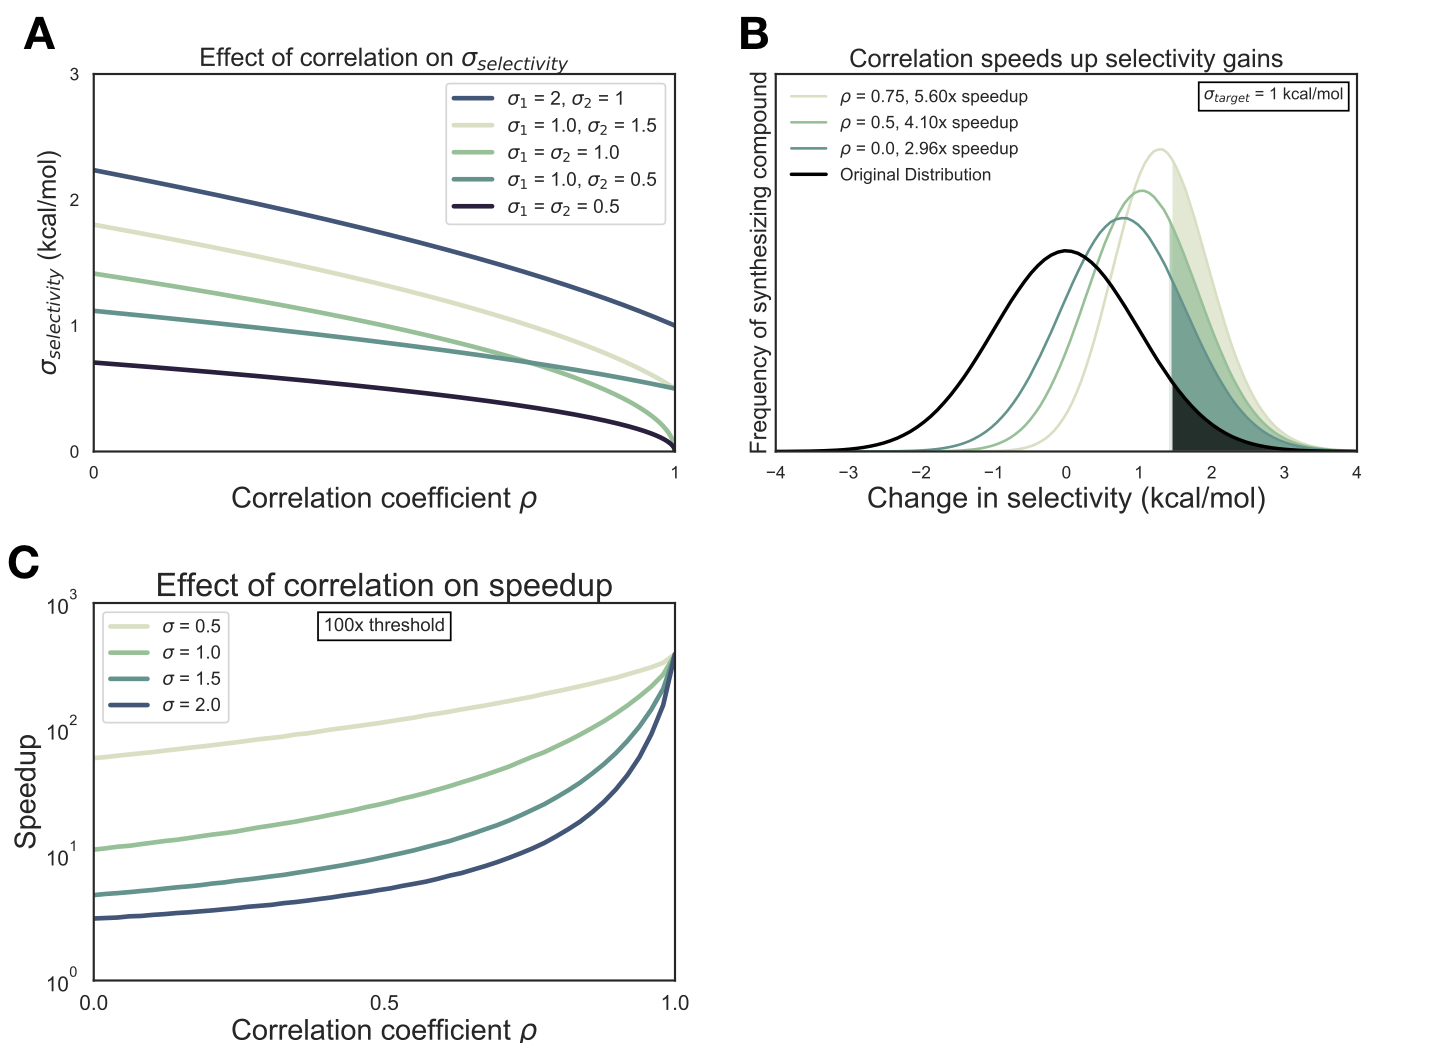
\includegraphics[width=1.0\linewidth]{figures/figure1.png}
% Need at least one blank line for centering to work.
\end{centering}
\caption{
\label{fig:figure-1}
{\bf Free energy calculations speed up selectivity optimization} \\
({\bf A})  The effect of correlation on expected errors for predicting selectivity ($\sigma_{selectivity}$) in kcal/mol. Each curve represents a different combination of target errors ($\sigma_1$ and $\sigma_2$). 
({\bf B}) The change in selectivity for molecules proposed by medicinal chemists optimizing a lead candidate can be modeled by a normal distribution centered on 0 with a standard deviation of 1 kcal/mol (black curve). Each green curve corresponds to the distribution of compounds made after screening for a 1 log unit (1.4 kcal/mol) improvement in selectivity with a free energy methodology with a 1 kcal/mol per target error and a particular correlation. The shade region of each curve corresponds to the compounds with a real 1 log unit  improvement in selectivity. The speed up is calculated as the ratio of the percentage of compounds made with a real 1 log unit improvement to the percentage of compounds that would be expected in the original distribution.  
({\bf C}) The speedup (y-axis, log scale) expected for 100x (2 log units, 2.8 kcal/mol) selectivity optimization as a function of correlation coefficient $\rho$. Each curve corresponds to a different $\sigma_{target}$ value.  
}
\end{fullwidth}
\end{figure}

\paragraph{The CDK2 and CDK9 experimental dataset demonstrates the difficulty in achieving selectivity for closely related kinases}

To begin quantifying the correlation of errors in free energy predictions for selectivity, we set out to gather datasets that met a number of criteria. We looked for datasets that contained binding affinity data for a number of kinase targets and ligands, as well as having crystal structures for each target with the same co-crystallized ligand. For the CDK2/CDK9 datatset~\citep{Shao2013-oe}, ligand 12c was cocrystallized with CDK2/cylin A (Figure~\ref{fig:figure-2}A, left) and CDK9/cyclin T (Figure~\ref{fig:figure-2}B, left), work that was published in a companion paper~\citep{Hole2013-sr}. In both CDK2 and CDK9, ligand 12c forms relatively few hydrogen bond interactions with the kinase. Each kinase forms a set of hydrogen bonds between the ligand scaffold and a hinge residue (C106 in CDK9 and L83 in CDK2) that is conserved across all of the ligands in this series. CDK9, which has slightly lower affinity for ligand 12c (Figure~\ref{fig:figure-2}C, right), forms a lone interaction between the sulfonamide of ligand 12c and residue E107. On the other hand, CDK2 forms interactions between the sulfonamide of ligand 12c and residues K89 and H84. The congeneric series of ligands contains a number of challenging perturbations, particularly at substituent point R3 (Figure~\ref{fig:figure-2}C, left). Ligand 12i also presented a challenging perturbation, moving the 1-(piperazine-1-yl)ethanone from the \emph{meta} to \emph{para} location. 

This congeneric series of ligands also highlights two of the challenges of working from publicly available data. First, the dynamic range of selectivity is incredibly narrow, with a mean $\Delta \Delta G_{selectivity}$ (CDK9 - CDK2) of only -0.65 kcal/mol, and a standard deviation of 0.88 kcal/mol. Additionally, experimental uncertainties are not reported for the experimental measurements. Thus, for this and subsequent sets of ligands, the experimental uncertainty is assumed to be 0.3 kcal/mol based on previous work done to summarize uncertainty in experimental data~\citep{BROWN2009420,Hauser:2018vz}. 

\begin{figure}
\begin{fullwidth}
\begin{centering}
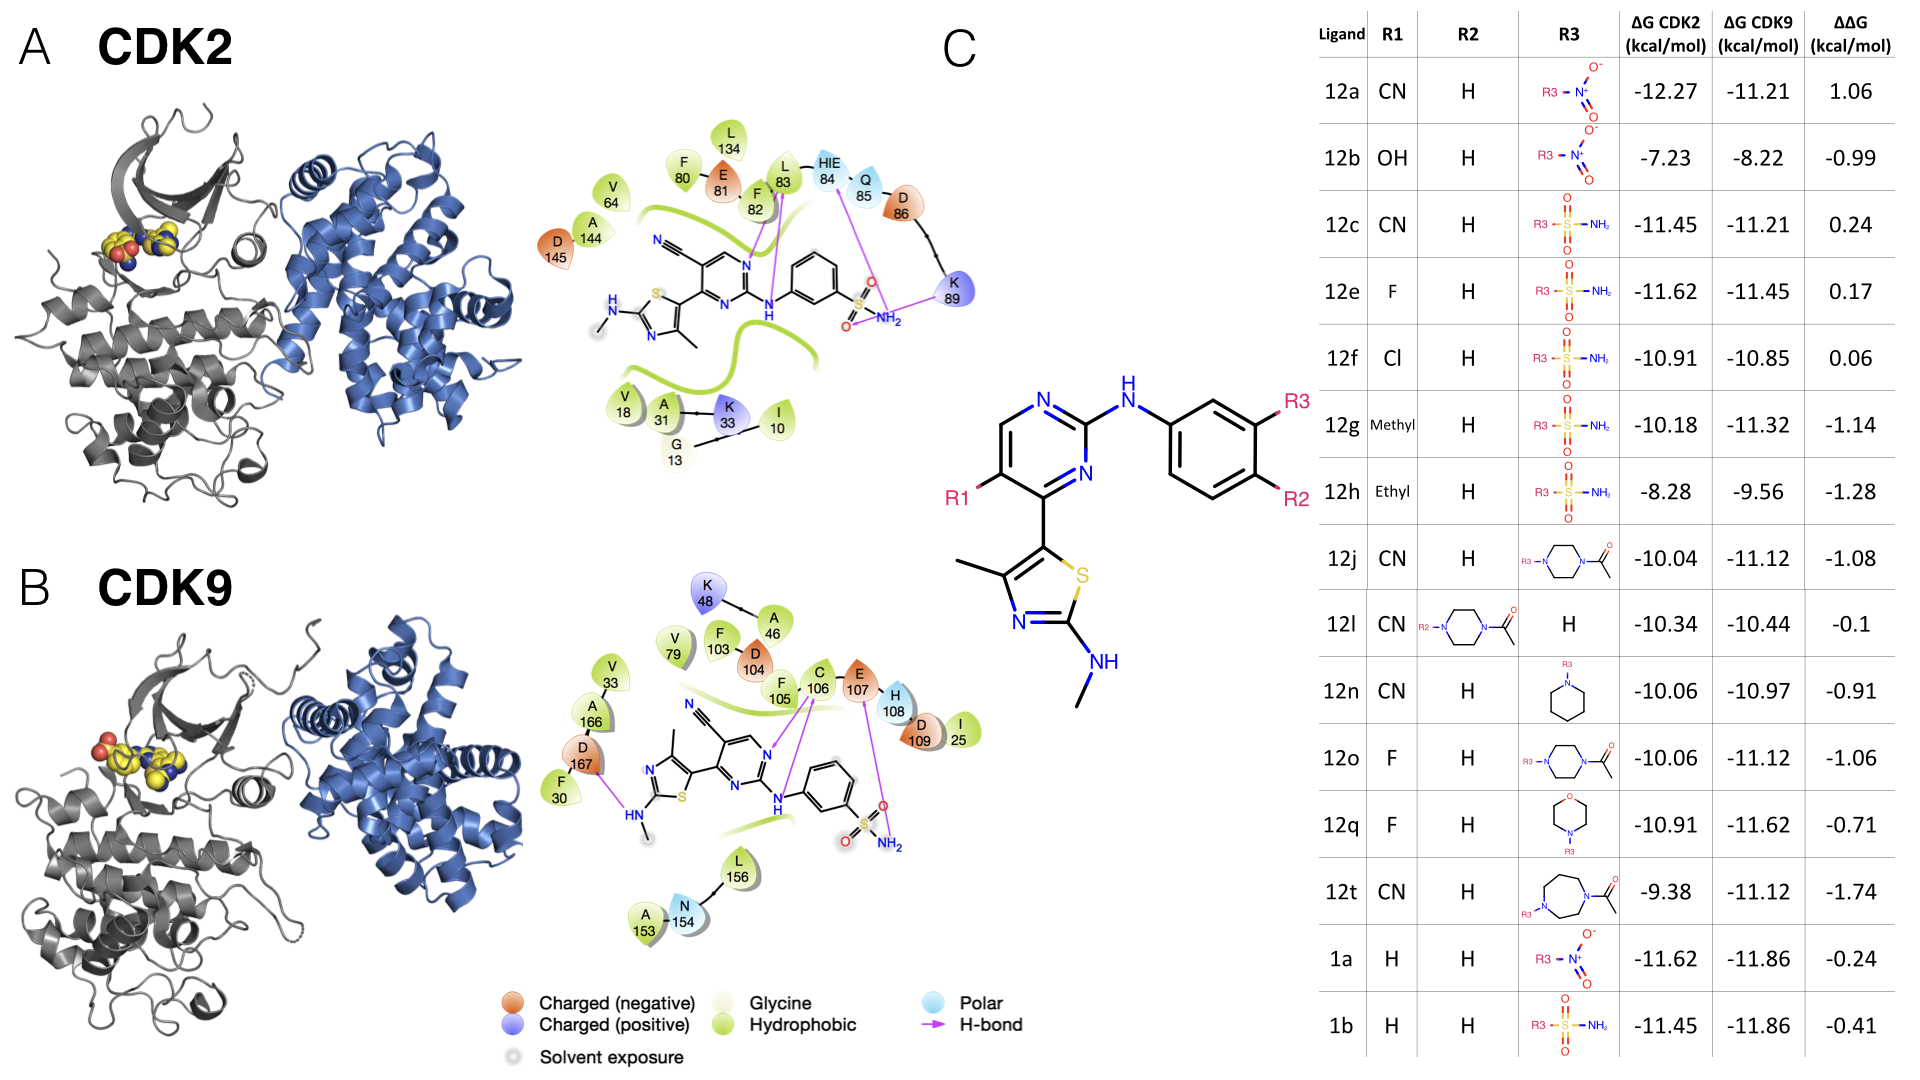
\includegraphics[width=1.0\linewidth]{figures/figure2.png}
% Need at least one blank line for centering to work.
\end{centering}
\caption{
\label{fig:figure-2}
{\bf A CDK2/CDK9 selectivity dataset from Shao et \emph{al}., 2013} \\
({\bf A})  \emph{(left)} Crystal Structure (4BCK)\citep{Hole2013-sr} of CDK2 (gray ribbon)  bound to ligand 12c (yellow spheres). Cyclin A is shown in blue ribbon \emph{(right)} 2D ligand interaction map of ligand 12c in the CDK2 binding site. 
({\bf B}) \emph{(left)} Crystal structure of CDK9 (4BCI)\citep{Hole2013-sr} (gray ribbon) bound to ligand 12c (yellow spheres). Cyclin T is shown in blue ribbon. \emph{(right)} 2D ligand interaction map of ligand 12c in the CDK9 binding site.
({\bf C}) \emph{(left)} 2D structure of the common scaffold for all ligands in congeneric ligand series 12 from the publication \emph{(right)} A table summarizing all R group substitutions as well as the published experimental binding affinities and selectivities\citep{Shao2013-oe}. 
}
\end{fullwidth}
\end{figure}

\paragraph{The CDK2 and ERK2 dataset achieves higher levels of selectivity for more distantly related kinases}
\todo{I probably need to either remove the reference to how closely related the kinases are, or come up with a way to quantify that - SKA}
The CDK2/ERK2 datatset from Blake \emph{et al.,} 2016 also met the criteria described above. Crystal structures for both CDK2 (Figure~\ref{fig:figure-3}A, top) and ERK2 (Figure~\ref{fig:figure-3}B, top) were available with ligand 22 co-crystallized. Of note, CDK2 was not crystallized with cyclin A, despite cyclin A being included in the affinity assay reported in the paper~\citep{Blake2016-su}. CDK2 adopts a DFG-in conformation with the $\alpha$C helix rotated out, away from the ATP binding site and breaking the conserved salt bridge between K33 and E51 (Supp. Figure~\ref{fig:sup-figure-1}A), indicative of an inactive kinase~\citep{Huse2002-ml,Hari:2013dp}. By comparison, the CDK2 structure from the CDK2/CDK9 dataset adopts a DFG-in conformation with the $\alpha$C helix rotated in, forming the ionic bond between K33 and E51 indicative of an active kinase, due to allosteric activation by cyclin A. While missing cyclins have caused problems for free energy calculations in prior work~\todo{is there a good citation for this?}, it is possible that the fully active conformation contributes equally to binding affinity for all of the ligands in the series, and the high accuracy of the potency predictions (Figure~\ref{fig:figure-4}, top left) is the result of fortutious cancellation of errors. The binding mode for this series is similar between both kinases. There is a set of conserved hydrogens bonds between the scaffold of the ligand and the backbone of one of the hinge residues (L83 for CDK2 and M108 for ERK2). The conserved lysine (K33 for CDK2 and K54 for ERK2), normally involved in the formation of a ionic bond with the $\alpha$C helix, forms a hydrogen bond with the scaffold (Figure~\ref{fig:figure-4}A and~\ref{fig:figure-4}B, bottom) in both CDK2 and ERK2. However, in the ERK2 structure, the hydroxyl engages a crystallographic water as well as N154 in a hydrogen bond network that is not present in the CDK2 structure. 
The congenric ligand series features a single subsituent point, with the R groups exposed to the solvent. This helps explain the extremely narrow distribution of selectivities, with a mean selectivity of -1.74 kcal/mol (ERK2 - CDK2) and standard deviation of 0.56 kcal/mol. This suggests that the selectivity is largely driven by the scaffold and unaffected by the R group substitutions.

\begin{figure}
\begin{fullwidth}
\begin{centering}
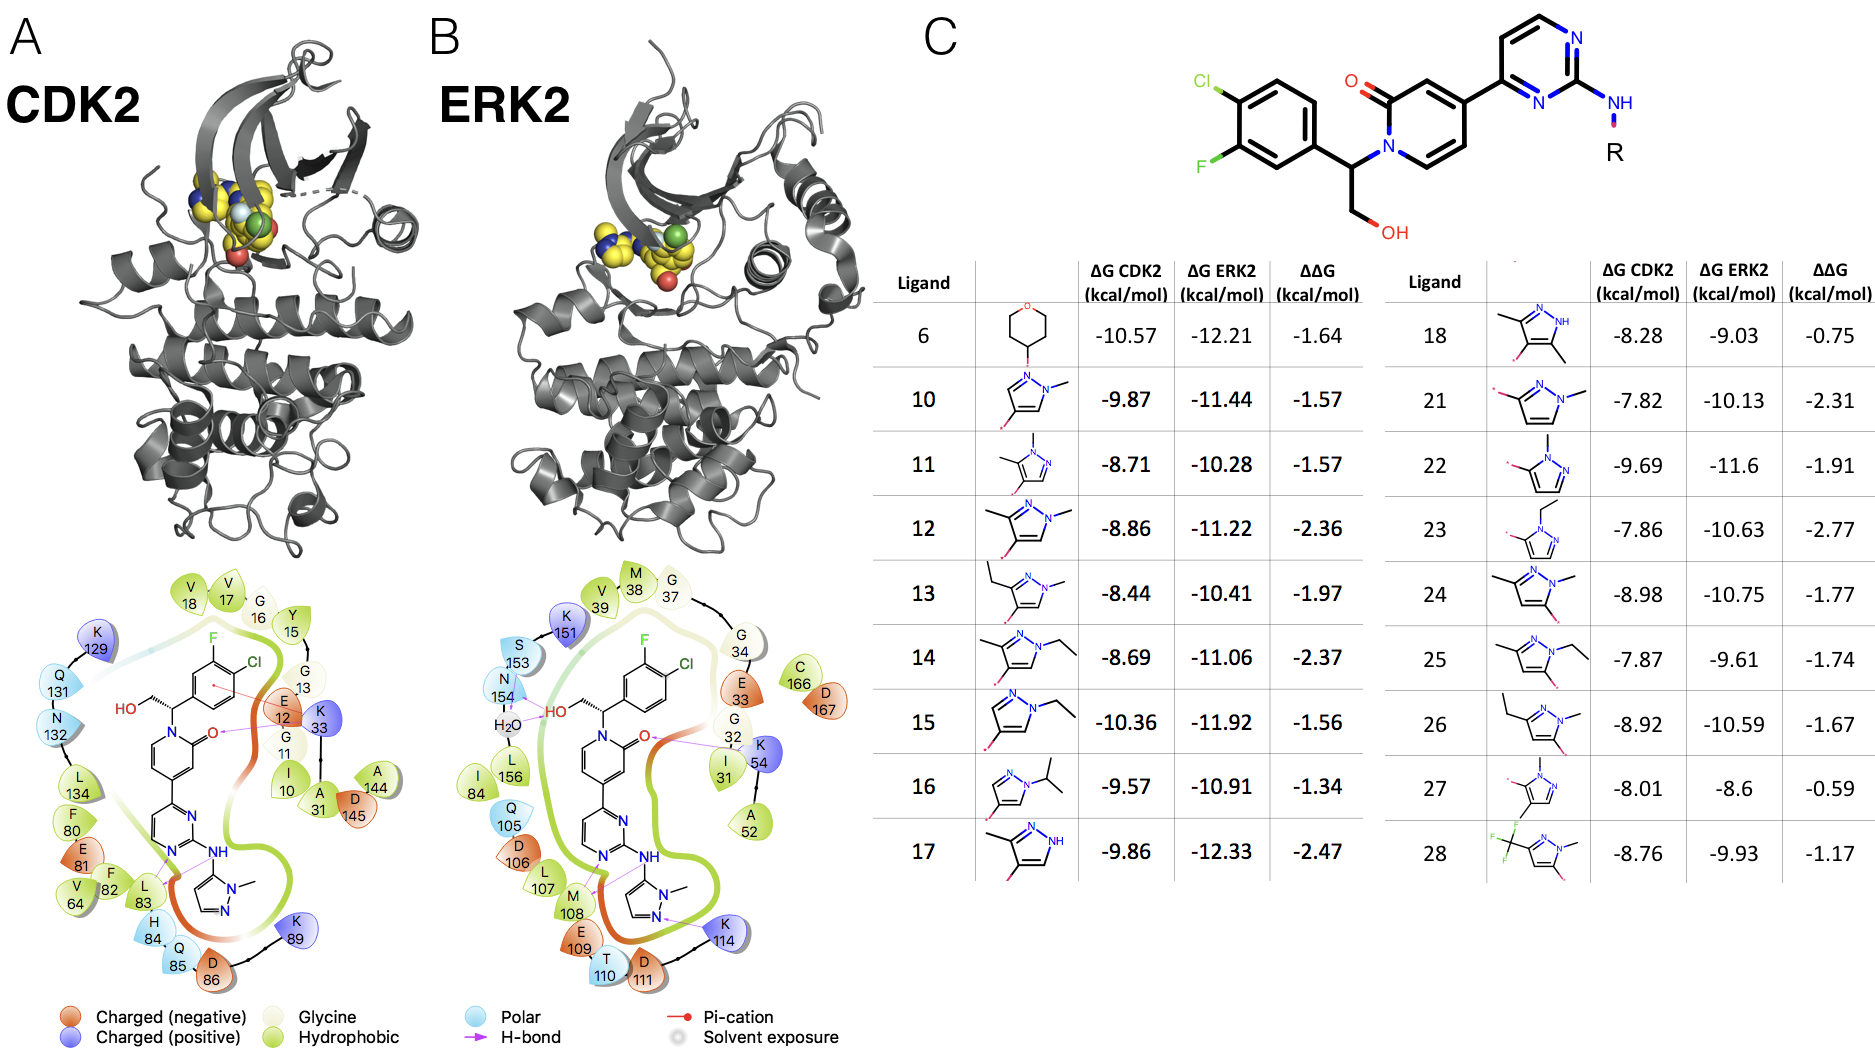
\includegraphics[width=1.0\linewidth]{figures/figure3.png}
% Need at least one blank line for centering to work.
\end{centering}
\caption{
\label{fig:figure-3}
{\bf CDK2 and ERK2 selectivity dataset from Blake et \emph{al}., 2016} \\
({\bf A})  \emph{(top)} Crystal structure of CDK2 (5K4J) shown in gray cartoon and ligand 22 shown in yellow spheres. \emph{(bot)} 2D interaction map of ligand 22 in the binding pocket of CDK2
({\bf B}) \emph{(top)} Crystal structure of ERK2 (5K4I) shown in gray cartoon with ligand 22 shown in yellow spheres. \emph{(bot)} 2D interaction map of ligand 22 in the binding pocket of ERK2.
({\bf C}) \emph{(top)} Common scaffold for all of the ligands in the Blake dataset, with R denoting attachment side for substitutions. \emph{(bot)} Table showing R group substitutions and experimentally measured binding affinities and selectivities. Ligand numbers correspond to those used in publication. 
}
\end{fullwidth}
\end{figure}

\paragraph{FEP+ calculations show accurate potency predictions for ERK2/CDK2 and larger errors for CDK2/CDK9}
The FEP+ predictions of single target potencies ($\Delta G$) showed good accuracy for the CDK2 and ERK2 dataset (Figure~\ref{fig:figure-4}, top), with an RMSE of $0.37^{0.57}_{0.16}$ and $0.53^{0.81}_{0.22}$ kcal/mol, respectively. All of the CDK2 and ERK2 potencies were predicted within 1 log unit of the experimental value. The selectivity ($\Delta \Delta G_{selectivity}$) predictions show an RMSE of $0.81^{1.26}_{0.37}$ kcal/mol, with all of the predictions falling within 1 log unit of the experimental values (Figure~\ref{fig:figure-4}, top right panel).\todo{this will change if we take of the ff uncertainty error bars}. Despite the high accuracy of the predictions, the narrow dynamic range and high uncertainty from experiment and calculation obscures any signal in the data. 
The CDK2 and CDK9 datasets show higher errors in the potency predictions, with an RMSE of $1.39^{2.05}_{0.58}$ and $1.71^{2.61}_{0.61}$ kcal/mol respectively. There are a number of outliers that fall outside of 1 log unit from the experimental value. While the higher per target errors make predicting potency more difficult, the selectivity predictions show a much lower RMSE of $0.74^{1.25}_{0.31}$ kcal/mol. This suggests that some correlation in the error is leading to fortuitous cancellation of systematic error, leading to more accurate than expected predictions of $\Delta \Delta G_{selectivity}$. 

\begin{figure}
\begin{fullwidth}
\begin{centering}
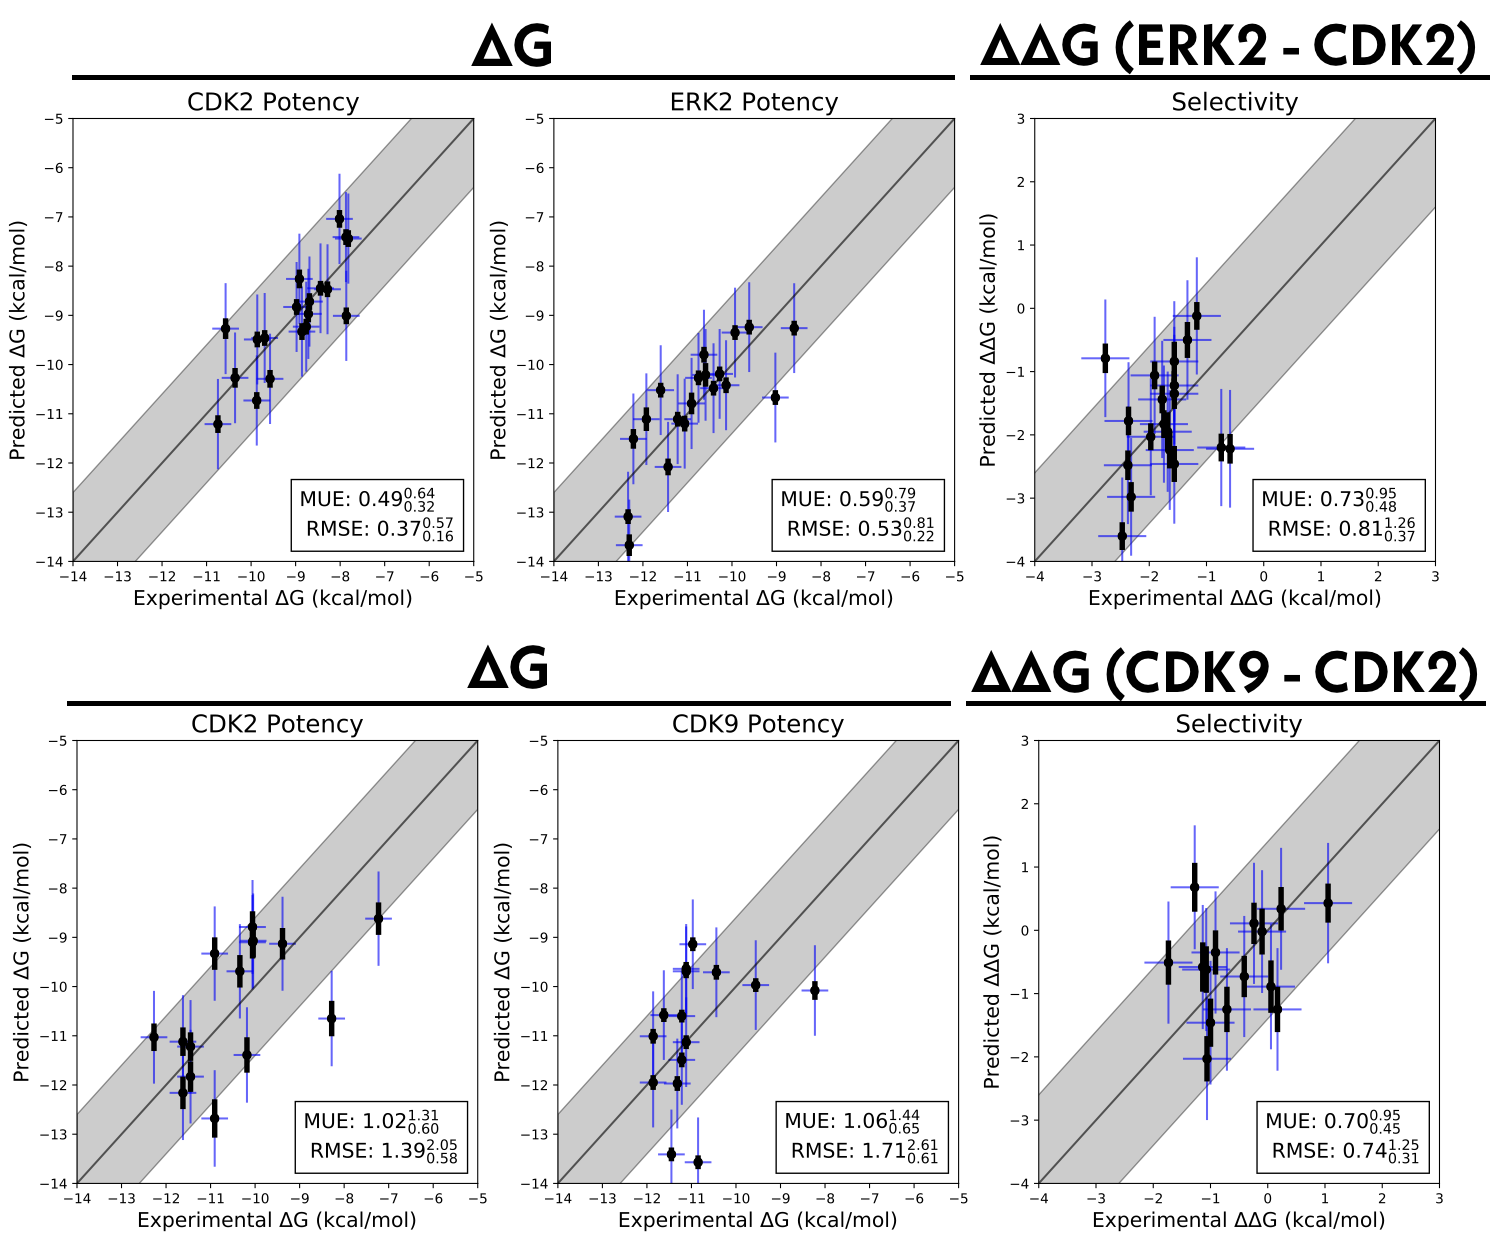
\includegraphics[width=1.0\linewidth]{figures/figure4.png}
% Need at least one blank line for centering to work.
\end{centering}
\caption{
\label{fig:figure-4}
{\bf Relative free energy calculations can accurately predict potency, but show larger errors for selectivity predictions.} \\
Single target potencies and selectivities for CDK2/ERK2 from the Blake datasets (\emph{top}), and CDK2/CDK9 (\emph{bottom}) from the Shao datasets. The experimental values are shown on the X-axis and calculated values on the Y-axis. Each data point corresponds to a ligand for a given target. All values are shown in units of kcal/mol. The horizontal error bars show the assumed experimental uncertainty of 0.3 kcal/mol\citep{BROWN2009420}. To better highlight outliers that are unlikely due simply to forcefield errors, we presume the forcefield error ($\sigma_\mathrm{FF} \approx$ 0.9 kcal mol$^{-1}$~\cite{Harder:J.Chem.TheoryComput.:2016}) also behaves as a random error. We show the total estimated statistical and forcefield error ($\sqrt{\sigma_\mathrm{FF}^2 + \sigma_\mathrm{calc}^2}$) as vertical blue error bars. The black vertical error bars correspond to the statistical error ($\sigma_{calc}$). The black line indicates agreement between calculation and experiment, while the gray shaded region represent 1.36 kcal/mol (or 1 log unit) error. The MUE and RMSE are shown on each plot with bootstrapped 95$\%$ confidence intervals.
}
\end{fullwidth}
\end{figure}

\paragraph{Correlation of forcefield errors accelerates selectivity optimization}
To quantify the correlation coefficient ($
\rho$) of the forcefield errors in our calculations, we built a Bayesian graphical model to separate the forecefield error from the statistical error, as described in the methods section. Briefly, we modeled the absolute free energy ($G$) of each ligand in each phase (complex and solvent) as in equation~\ref{eq4}. The model was chained to the FEP+ calculations by providing the $\Delta G^{calc}_{phase,ij,target}$ as observed data, as in equation~\ref{eq6}. As in equation, the experimental data was modeled as a normal distribution centered around the true free energy of binding ($\Delta G^{true}_{i,target}$) corrupted by experimental error, which is assumed to be 0.3 kcal/mol from previous work done to quantify the uncertainty in publicly available data~\citep{BROWN2009420}. The reported IC50 values from each dataset were treated as data observations (Equation~\ref{eq12}) and the $\Delta G^{true}_{i,target}$ was assigned a weak normal prior (Equation~\ref{eq13}). The correlation coefficient was calculated for each sample according to equation~\ref{eq9}. 
The correlation coefficient $\rho$ for the CDK2/ERK2 calculations was quantified to be $0.5^{0.33}_{-0.23}$, indicating that the errors are largely uncorrelated between ERK2 and CDK2 (Figure~\ref{fig:figure-5}A, right). The joint marginal distribution of the error ($\epsilon$) for each target is symmetric, which is expected for cases in which $\rho$ is 0 (Supp. Figure~\ref{fig:sup-figure-2}). Despite the weak correlation in errors, the high per target accuracy of these calculations should have a 2-3x speed up for 1 log unit selectivity optimization, and a 20-30x speed up for 2 log unit selectivity optimization (Figure~\ref{fig:figure-5}A, right). 
The CDK2/CDK9 calculations show strong evidence of correlation, with a correlation coefficient of $0.70^{0.82}_{0.57}$ (Figure~\ref{fig:figure-5}B, right). The joint marginal distribution of errors is strongly diagonal, which is expected based on the value for $\rho$ (Figure~\ref{fig:figure-5}B, left). The high correlation in errors leads to a speed up of 4-5 for 1 log unit selectivity optimization and 30-40x for 2 log unit selectivity optimization (Figure~\ref{fig:figure-5}B, right), despite the much higher per target errors.
Quantifying $\rho$ for these calculations enables estimation of $\sigma_{selectivity}$, which is useful for estimating expected error for prospective studies, where the experimental values for $\Delta \Delta G_{selectivity}$ are not yet known. Based on the distribution quantified for $\rho$, the expected $\sigma_{selectivity}$ for the CDK2/CDK9 calculations is between 0.76 and 1.16 kcal/mol (Supp. Figure~\ref{fig:sup-figure-3}), which is in good agreement with the bootstrapped RMSE (Figure~\ref{fig:figure-4}, bottom). For the CDK2/ERK2 calculations, $\sigma_{selectivity}$ is expected to fall between 0.82 kcal/mol and 1.10 kcal/mol (Supp. Figure~\ref{fig:sup-figure-3}), which is also in good agreement with the bootstrapped RMSE (Figure~\ref{fig:figure-4}, top). 





\begin{figure}
\begin{fullwidth}
\begin{centering}
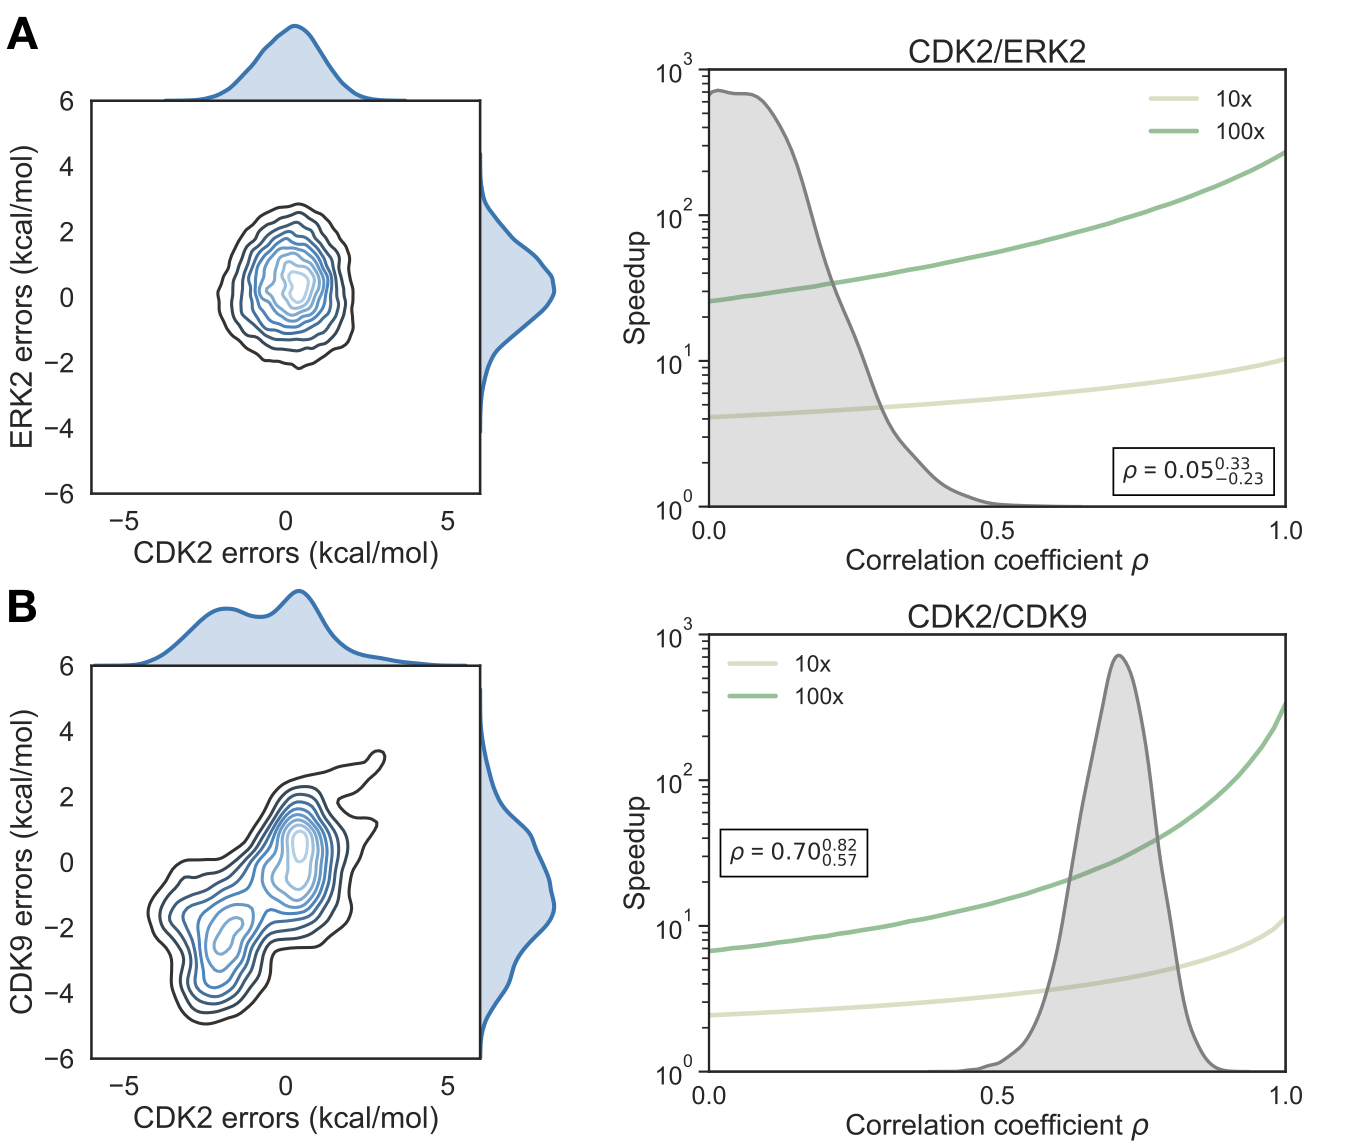
\includegraphics[width=1.0\linewidth]{figures/figure5.png}
% Need at least one blank line for centering to work.
\end{centering}
\caption{
\label{fig:figure-5}
{\bf Correlation in selectivity prediction errors can be used to accelerate selectivity optimization} \\
({\bf A}) (\emph{left}) The joint posterior distribution of the prediction errors for CDK2 (X-axis) and ERK2 (Y-axis) from the Bayesian graphical model. (\emph{right}) Speedup in selectivity optimization (Y-axis) as a function of correlation coefficient (X-axis). The posterior marginal distribution of the correlation coefficient ($\rho$) is shown in gray, while the expected speed up is shown for 100x (green curve) and 10x (yellow curve) selectivity optimization. The inserted box shows the mean and 95\% confidence interval for the correlation coefficient. 
({\bf B}) (\emph{left}) The same as above, with CDK2 (X-axis) and CDK9 (Y-axis). (\emph{right}) As above, for the CDK2/CDK9 calculations.}
\end{fullwidth}
\end{figure}


%
%
%  Discussion and Conclusions 
%
%
\section{Discussion and Conclusions}
We have demonstrated, using a simple numerical model, the impact that free energy calculations with even weakly correlated errors can have on speeding up the optimization of selectivity in small molecule kinase inhibitors. While the expected speed up is dependent on the per target error of the method ($\sigma_{target}$), the speedup is also highly dependent on the correlation of errors made for both targets. Unsurprisingly, free energy methods have greater impact as the threshold for selectivity optimization goes from 10x to 100x. While 100x selectivity optimization is difficult to achieve, the expected benefit from free energy calculations is also quite high, with 1 and 2 order of magnitude speedups possible. 
To quantify the correlation of errors in two example systems, we gathered experimental data for two congeneric ligand series with experimental data for CDK2 and ERK2, as well as CDK2 and CDK9. These datasets, which had crystal structures for both targets with the same ligand co-crystallized, exemplify the difficulty in predicting selectivity. The dynamic range of selectivity for both systems is incredibly narrow, with most of the perturbations not having a major impact on the overall selectivity achieved. Further, the data was reported with unrelaible experimental uncertainties, which makes quantifying the errors made by the free energy calculations difficult. This issue is common when considering selectivity, as many kinase-oriented high throughput screens are carried out at a single concentration and not highly quantitative. 
\todo[inline]{discuss quantification of rho (is there a way to know a priori what rho might be?)}
\todo[inline]{discussion of the expected speedup and sigma based on the quantification of rho}
\todo[inline]{extensions include: separating statistical error (unless this gets added into the results section}

%
\newpage
%



%%%%%%%%%%%%%%%%%%%%%%%%%%%%%%%%%%%%%%%%%%%%%%%%%%%%%%%%%%%%
%%% ACKNOWLEDGMENTS
%%%%%%%%%%%%%%%%%%%%%%%%%%%%%%%%%%%%%%%%%%%%%%%%%%%%%%%%%%%%

\section{Acknowledgments}
JDC and SKA acknowledge support from NIH grant R01 121505.
JDC acknowledges partial support from NIH grant P30 CA008748.

\textbf{To be filled out soon}


\section{Disclosures}

JDC was a member of the Scientific Advisory Board for Schrödinger, LLC during part of this study.
JDC is a current member of the Scientific Advisory Board of OpenEye Scientific Software.
The Chodera laboratory receives or has received funding from multiple sources, including the National Institutes of Health, the National Science Foundation, the Parker Institute for Cancer Immunotherapy, Relay Therapeutics, Entasis Therapeutics, Silicon Therapeutics, EMD Serono (Merck KGaA), AstraZeneca, XtalPi, the Molecular Sciences Software Institute, the Starr Cancer Consortium, the Open Force Field Consortium, Cycle for Survival, a Louis V. Gerstner Young Investigator Award, and the Sloan Kettering Institute.
A complete funding history for the Chodera lab can be found at http://choderalab.org/funding

%%%%%%%%%%%%%%%%%%%%%%%%%%%%%%%%%%%%%%%%%%%%%%%%%%%%%%%%%%%%
%%% AUTHOR CONTRIBUTIONS
%%%%%%%%%%%%%%%%%%%%%%%%%%%%%%%%%%%%%%%%%%%%%%%%%%%%%%%%%%%%

\section{Author Contributions}
Conceptualization: SKA, LW, RA, JDC \\
Methodology: SKA, LW, JDC\\
Investigation: SKA, SP\\
Writing -- Original Draft: SKA\\
Writing -- Review \& Editing: SKA, JDC \\
Funding Acquisition: RA, JDC\\
Resources: LW, JDC\\
Supervision: LW, JDC


%
\newpage
%





%%%%%%%%%%%%%%%%%%%%%%%%%%%%%%%%%%%%%%%%%%%%%%%%%%%%%%%%%%%%
%%% BIBLIOGRAPHY
%%%%%%%%%%%%%%%%%%%%%%%%%%%%%%%%%%%%%%%%%%%%%%%%%%%%%%%%%%%%

%\nocite{*} % This command displays all refs in the bib file
%\bibliography{zotero}
%
%  FIXME
%
\bibliography{albanese} %zotero + new citations HK added manually.



%
%
\newpage
%
%





%%%%%%%%%%%%%%%%%%%%%%%%%%%%%%%%%%%%%%%%%%%%%%%%%%%%%%%
%%%%%%%%%%%%%%%%%%%%%%%%%%%%%%%%%%
%%%%%%%%%%%%%%%%%%%%%
%%%%%%%%%%%%%
%%%%%%%%
%%%%%
%%%
%%
%
%
%
%
%    Supplementary Information
%
%
\newpage
\section{Supplemental Information}
\setcounter{figure}{0} 
\renewcommand{\figurename}{Supplemental Figure.}

\begin{figure}[h]
\begin{fullwidth}
\begin{centering}
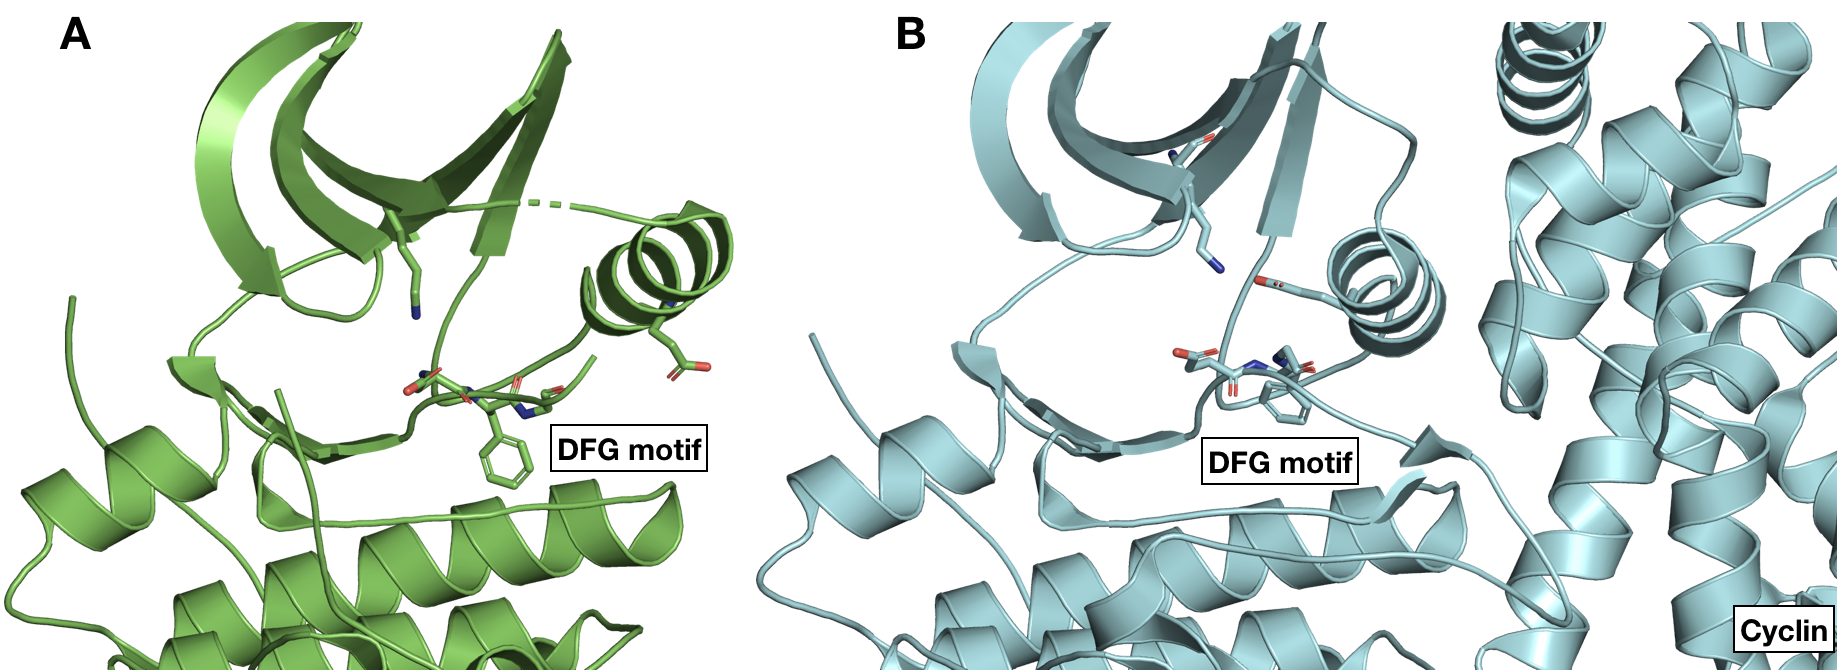
\includegraphics[width=1.0\linewidth]{figures/supp_figure1.png}
% Need at least one blank line for centering to work.
\end{centering}
\caption{
\label{fig:sup-figure-1}
{\bf CDK2 adopts an inactive conformation in the crystal structure used for the CDK2/ERK2 calculations} \\
({\bf A}) CDK2 (5K4J) adopts an inactive conformation in the absence of its cyclin. The DFG motif is in a DFG-in conformation, with the $\alpha$C helix rotated outwards, breaking the salt bridge between K33 and E51 (Uniprot numbering) that is typically a marker of an active conformation. Notably, the Phe in the DFG motif does not completely form the hydrophobic spine due to the rotation of the $\alpha$C helix~\citep{Hu:2015kh}
({\bf B}) The CDK2 structure used for the CDK2/CDK9 calculations (4BCK) contains cyclin A and adopts a DFG-in/$\alpha$C helix-in conformation that forms the salt bridge between K33 and E51. This is typically indicative of a fully active kinase~\citep{Huse2002-ml,Hari:2013dp}. 
}
\end{fullwidth}
\end{figure}

\begin{figure}[h]
\begin{fullwidth}
\begin{centering}
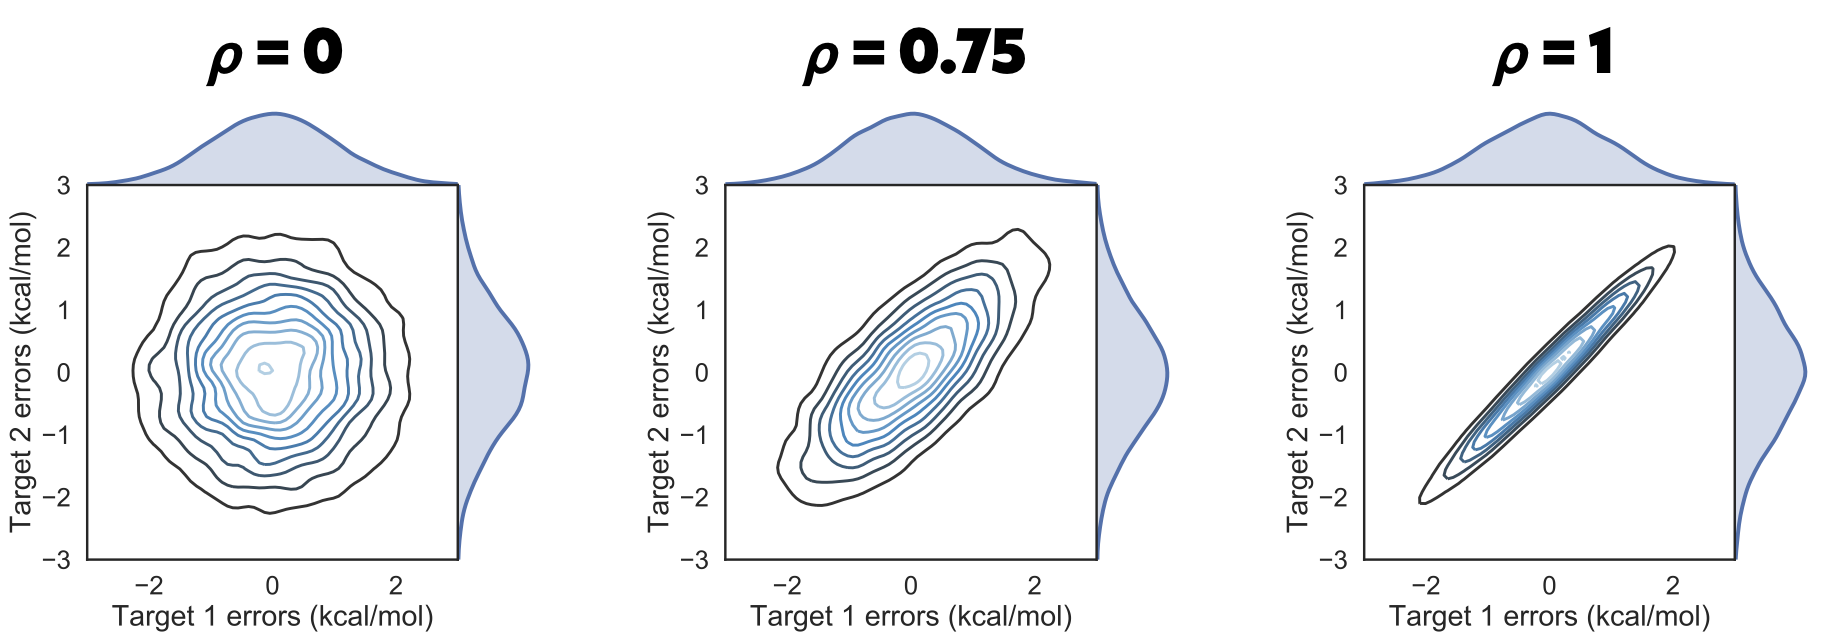
\includegraphics[width=1.0\linewidth]{figures/supp_2.png}
% Need at least one blank line for centering to work.
\end{centering}
\caption{
\label{fig:sup-figure-2}
{\bf Correlation coefficient $\rho$ controls the shape of the joint marginal distribution of errors} \\
As $\rho$ increases, the joint marginal distribution of errors become more diagonal. Each panel shows 10000 samples drawn from a multivariate normal distribution centered around 0 kcal/mol, where the per target error was set to 1 kcal/mol and $\rho$ to the value indicated in bold over the plot. 
}
\end{fullwidth}
\end{figure}

\begin{figure}[h]
\begin{fullwidth}
\begin{centering}
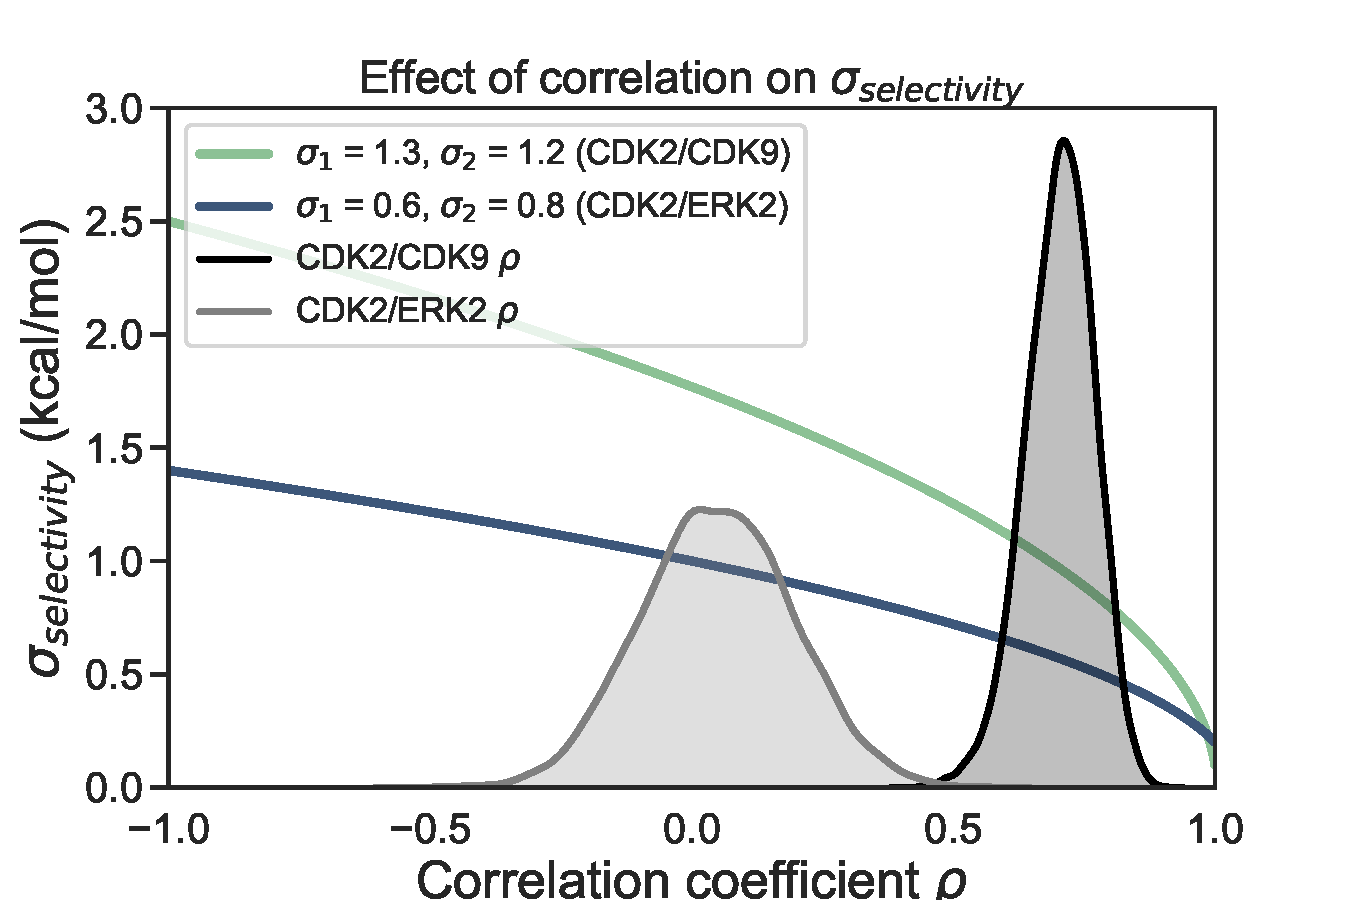
\includegraphics[width=1.0\linewidth]{figures/supp_figure3.pdf}
% Need at least one blank line for centering to work.
\end{centering}
\caption{
\label{fig:sup-figure-3}
{\bf Correlation reduces the expected error for selectivity predictions} \\
As corelation coefficient $\rho$ increases, $\sigma_{selectivity}$ decreases. The intersection between CDK2/CDK9 $\sigma_{selectivity}$ (green curve) and $\rho$ (black distribution) indicates the range of expected $\sigma_{selectivity}$ values. The intersection for CDK2/ERK $\sigma_{selectivity}$ (blue curve) and $\rho$ (gray distribution) suggests the expected $\sigma_{selectivity}$ range for that set of calculations. 
}
\end{fullwidth}
\end{figure}


%%%%%%%%%%%%%%%%%%%%%%%%%%%%%%%%%%%%%%%%%%%%%%%%%%%%%%%%%%%
%%%%%%%%%%%%%%%%%%%%%%%%%%%%%%%%%%%%%%%%%%%%%%%%%%%%%%%%%%%
%\fi
%%%%%%%%%%%%%%%%%%%%%%%%%%%%%%%%%%%%%%%%%%%%%%%%%%%%%%%%%%%
%%%%%%%%%%%%%%%%%%%%%%%%%%%%%%%%%%%%%%%%%%%%%%%%%%%%%%%%%%%




\end{document}
%%%%%%%%%%%%%%%%%%%%%%%%%%%%%%%%%%%%%%%%%%%%%%%%%%%%%%%%%%%%%%%%%%%%%%%%%%%%%%%%%%%%%%%%%%%%%%%%%%%%%%%%%%%%%%%%%%%%%%%%%%%%%%%%%%%%%%%%%%%%%%%%
%%%%%%%%%%%%%%%%%%%%%%%%%%%%%%%%%%%%%%%%%%%%%%%%%%%%%%%%%%%%%%%%%%%%%%%%%%%%%%%%%%%%%%%%%
%%%%%%%%%%%%%%%%%%%%%%%%%%%%%%%%%%%%%%%%%%%%%%%%%%%%%%%
%%%%%%%%%%%%%%%%%%%%%%%%%%%%%%%%%%
%%%%%%%%%%%%%%%%%%%%%
%%%%%%%%%%%%%
%%%%%%%%
%%%%%
%%%
%%
%
%
